\documentclass[12pt]{article}
\usepackage[a4paper, width=6.3in, left=1.3in, right=1.3in, height=9.2in, top=1.1in]{geometry}
\usepackage{amsfonts,amsmath,amssymb,amsthm}
\usepackage[none]{hyphenat}
\usepackage{fancyhdr}
\usepackage[nottoc,notlot,notlof]{tocbibind}
\usepackage{verbatim}
\usepackage{graphicx}
\usepackage{wrapfig}
\usepackage{caption}
\usepackage[table]{xcolor}
\fancyfoot[R]{\thepage}
\usepackage{listings}
\usepackage{ctable}
\usepackage{color} %red, green, blue, yellow, cyan, magenta, black, white
\usepackage[title, titletoc]{appendix}
\usepackage{array}
\usepackage{hyperref}
\usepackage{cleveref}

\newcolumntype{C}[1]{>{\centering\arraybackslash}p{#1}}

\definecolor{mygreen}{RGB}{28,172,0} % color values Red, Green, Blue
\definecolor{mylilas}{RGB}{170,55,241}
\definecolor{mygrey}{RGB}{123,123,123}


\newcommand{\mbeq}{\overset{!}{=}}

\newcommand{\einsch}{\,\rule[-5pt]{0.4pt}{15pt}\,{}}
\parindent 0ex
\renewcommand{\baselinestretch}{1.5}
\newtheorem{assumption}{Assumption}[section]
\newtheorem{theorem}{Theorem}[section]
\newtheorem{lemma}[theorem]{Lemma}
\newtheorem{notation}[theorem]{Notation}
\newtheorem{remark}[theorem]{Remark}
\newtheorem{definition}[theorem]{Definition}
\renewcommand{\labelenumi}{\em{(\roman{enumi})}}
\renewcommand{\labelenumii}{\em{(\alph{enumii})}}
\captionsetup[figure]{skip=0pt}


\begin{document}
	\begin{titlepage}
		
		
		
		\begin{center}
			\normalsize{Ludwig-Maximilians-Universität München \\
				Mathematisches Institut}\\[15ex]
			
			\LARGE{Master's Thesis}\\[1.2ex]	
			\LARGE{\textbf{Default Forward Rate Models for the Valuation of Loans including Behavioral Aspects}} \\[2.5ex]
			\Large{\textit{Markus Parhofer}}\\[9ex]
		\end{center}
		
		
		\begin{center}
			
\includegraphics[width=1.8in]{siegel}\\[13ex]
		\end{center}
		
		\begin{center}
			\normalsize{}
			Under supervision of\\
			Prof. Dr. Christian Fries\\
			\today\
			\\
		\end{center}
		
	
	
	
\end{titlepage}

\tableofcontents
\thispagestyle{empty}
\clearpage


	
	
	% ------------------------------Content------------------------
	
	
	% ----------- Intro -----------
	
	
	
	\section{Introduction}
	\subsection{Motivation}
	\subsection{Aim of the thesis}
	\subsection{Preliminaries}
	The thesis is aimed at an audience that has a deep analytical background and a basic knowledge in stochasticity and financial mathematics.\\
	\color{red}If one has knowledge in the following areas, it is a good start:\color{black}
	\begin{itemize}
		\item Brownian-Motions and martingales,
		\item stochastic integration,
		\item Itô stochastic processes,
		\item definition of and theorems on arbitrage freeness.
	\end{itemize}
	Furthermore we assume a fundamental understanding of what these mathematical concepts imply on the real world and the other way around: How are the mathematical concepts motivated by the economical world?
	
	
	
	
	% --------------------------- Fundamentals----------------------
	
	
	
	\pagebreak
	\section{Fundamentals}
	In this section we provide some fundamentals for the thesis. Many of the results mentioned here can also be found in different versions in other scientific papers. We will stick to source 
	\color{red}[Add source] \color{black} %TODO: Add source
	for more application-oriented and source 
	\color{red}[Add source] \color{black} %TODO: Add source
	for more theoretical results.
	
	\subsection{Probability Theory}
	In our whole thesis we will assume a filtered probability space
	\begin{align*}
		(\Omega, \mathcal{F}, \mathbb{F}, \mathbb{Q})
	\end{align*}
	where
	\begin{itemize}
		\item $\Omega$ is the set of all states,
		\item $\mathcal{F}$ is a $\sigma$-algebra,
		\item $\mathbb{F} = (\mathcal{F}_t)_{t \in \left[0;\tilde{T}\right]}$ is a filtration with $\mathcal{F}_t \subset \mathcal{F} \quad \forall t \in [0;\tilde{T}]$, $\mathcal{F}_0 = \{\Omega, \emptyset \}$ and
		\item $\mathbb{Q}$ is a probability measure on $\mathcal{F}$.
	\end{itemize}
	Let us cover some notations.
	\begin{notation}
		Let $X$ and $Y$ be Itô stochatic processes and $W$ be a Brownian-Motion with:
		\begin{align*}
			X_t &= X_0 + \int_{0}^{t}\mu^X_s ds + \int_{0}^{t}\phi_s dW_s, \\
			Y_t &= Y_0 + \int_{0}^{t}\mu^Y_s ds + \int_{0}^{t}\psi_s dW_s.
		\end{align*}
		The \emph{sharp bracket} or \emph{quadratic variation} of $X$ is 
		\begin{align*}
			\left\langle X \right\rangle_t = \int_{0}^{t}\phi_s^2 ds.
		\end{align*}.
		The \emph{quadratic covariation} of $X$ and $Y$ is 
		\begin{align*}
			\left\langle X, Y \right\rangle_t = \int_{0}^{t}\phi_s \psi_s ds.
		\end{align*}
		For a $n$-dimensional Brownian-Motion $W = (W^i)_{i\in\{1,...,n\}}$ and therefore $n$-dimensional diffusion processes $\phi=(\phi^i)_{i \in \{1,..., n\}}$, $\psi=(\psi^i)_{i \in \{1,..., n\}}$ the quadratic covariation is
		\begin{align*}
			\left\langle X, Y \right\rangle_t = \sum_{i=1}^{n} \int_{0}^{t} \phi^i_s \psi^i_s ds
		\end{align*}
	\end{notation}
	For convenience we state a formula for stochastic integration by parts and a extended version of Itô's theorem:
	\begin{lemma}
		Let $X$ and $Y$ be two Itô stochastic processes. Then
		\begin{align*}
			X_t Y_t = X_0 Y_0 + \int_{0}^{t}X_sdY_s + \int_{0}^{t}Y_sdX_s + \left\langle X, Y\right\rangle_t
		\end{align*}
	\end{lemma}
	\begin{proof}
		See \cite{fima2Lecture}.
	\end{proof}
	\begin{theorem}
		Let $X$ be an Itô stochastic process, $f: \mathbb{R}^n \times [0;\tilde{T}] \rightarrow \mathbb{R}, \; (x,t) \rightarrowtail f(x, t)$ be two times differentiable in $x$ and differentiable in $t$. Then
		\begin{align*}
			f(X_t, t) = \;&f(X_0, 0) + \int_{0}^{t}(\partial_{t}f)(X_s, s)ds + \sum_{i=1}^{n}\int_{0}^{t}(\partial_{x^i}f)(X_s, s)dX^i_s \\
			&+ \frac{1}{2} \sum_{i,j=1}^{n}\int_{0}^{t}(\partial^2_{x^ix^j}f)(X_s, s)d\left\langle X^i, X^j\right\rangle_s
		\end{align*}
		
	\end{theorem}
	\begin{proof}
		See \cite{fima2Lecture}.
	\end{proof}
	
	Through Itô's formula we can prove the following statement.
	\begin{lemma}\label{lm:logNormalDyn}
		Let $W=(W^i)_{i\in \{1, ..., d\}}$ be a d-dimensional Brownian Motion, $\mu$ be a 1- dimensional and $\sigma = (\sigma^i)_{i\in \{1, ..., d\}}$ a $d$-dimensional stochastic process. Let following stochastic differential equation (SDE) be given:
		\begin{align}\label{eq:lognormalSDE}
			\begin{aligned}
				dY_t = Y_t \mu_t dt + Y_t \sigma_t \cdot dW_t,\\
				Y_0 = y,
			\end{aligned}
		\end{align}
		where $y > 0$.\\
		Then solving \cref{eq:lognormalSDE} is equivalent to solving
		\begin{align}\label{eq:lognormalSDENormalized}
			\begin{aligned}
				Y_t = \exp(X_t),\\
				dX_t = (\mu_t - \frac{1}{2}\sum_{i=1}^{d}(\sigma^i_t)^2)dt + \sigma_t \cdot dW_t,\\
				X_0 = \log(y).
			\end{aligned}
		\end{align}
	\end{lemma}
	\begin{proof}
		We use Itô's formula on \cref{eq:lognormalSDENormalized} with $f(x) = \exp(x)$, hence 
		\begin{align*}
			(\partial_xf)(x) = \exp(x), \quad (\partial^2_{xx})(x) = \exp(x).
		\end{align*}
		We get (in SDE format):
		\begin{align*}
			dY_t &= d\exp(X_t) = \exp(X_t)dX_t + \frac{1}{2}\exp(X_t)d\left\langle X \right\rangle_t\\
			&=	Y_t((\mu_t -\frac{1}{2}\sum_{i=1}^{d}(\sigma^i_t)^2)dt + \sigma_t \cdot dW_t) + \frac{1}{2}Y_t \sum_{i=1}^{d}(\sigma^i_t)^2 dt\\
			&= Y_t \mu_t dt + Y_t \sigma_t \cdot dW_t,
		\end{align*}
		which yields \cref{eq:lognormalSDE}.
	\end{proof}
	\begin{remark}
		It is easy to see, that because of the relation 
		\begin{align*}
			Y_t = \exp(X_t),
		\end{align*}
		it holds that $Y_t > 0 \quad \forall t \in [0;\tilde{T}]$.
	\end{remark}
	
	
	\subsection{Factor Loadings}\label{sec::FactorLoading}
	The problem we face in this section is that of correlated Brownian-Motions. \\
	Assume we have two SDEs for stochastic processes $X$ and $Y$:	
	\begin{align*}
		dX_t = \mu^X_t dt + \sigma^X_t dW^{\mathbb{Q}, 1}_t,\\
		dY_t = \mu^Y_t dt + \sigma^Y_t dW^{\mathbb{Q}, 2}_t,
	\end{align*}
	where $W^{\mathbb{Q}, 1}$ and $W^{\mathbb{Q}, 2}$ are instantaneously correlated Brownian-Motions under the same measure $\mathbb{Q}$. This correlation $\rho$ is expressed by a quadratic covariation of the Brownian-Motions \cite{FriesBook}:
	\begin{align*}
		\left\langle W^{\mathbb{Q}, 1}, W^{\mathbb{Q}, 2} \right\rangle_t = \int_{0}^{t}\rho_s ds
	\end{align*}
	or as SDE:
	\begin{align*}
		d\left\langle W^{\mathbb{Q}, 1}, W^{\mathbb{Q}, 2} \right\rangle_t = \rho_t dt.
	\end{align*}
	However implementation-wise we need to simulate SDEs using only independent Brownian-Motions. For this purpose we will take advantage of the properties of a Brownian-Motion. Recall following Lemmatas:
	\begin{lemma}
		$W = (W^i)_{i\in\{1, ..., d\}}$ is a $d$-dimensional Brownian-Motion if and only if $W^1, ..., W^d$ are independent 1-dimensional Brownian-Motions
	\end{lemma}
	\begin{proof}
		See \cite{fima2Lecture}.
	\end{proof}
	\begin{lemma}
		For any $d$-dimensional Brownian-Motion $W = (W^i)_{i\in\{1, ..., d\}}$ and weights $(a_i)_{i\in\{1,...d\}}$ with $a_1 + ... + a_d = 1$ it holds, that $U$ given by:
		\begin{align*}
			U_t = \sum_{i=1}^{d}a_iW^i_t
		\end{align*}
		is also a Brownian-Motion.
	\end{lemma} 
	\color{red}Elaborate!!!\color{black}. 
	%TODO: Elaborate
	
	
	\pagebreak
	\section{LIBOR Market Model}\label{sec::LIBORModel}
	
	While the actual LIBOR, short for "London Inter-Bank Offered Rate" \color{red}[Add source] \color{black} %TODO: Add source
	lost most of its influence after the banking crash of 2008 \color{red}[Add source] \color{black} %TODO: Add source
	the LIBOR market model - or discrete forward rate model - is still a very popular mathematical model for simulation and valuation of financial products on fixed income markets.\\
	The idea of the model  \color{red}Elaborate!!!\color{black}. 
	%TODO: Elaborate
	\\
	The basic assumption of the LIBOR Market Model is that we are in an arbitrage free and complete market.
	
	\subsection{Fixed Income Markets Terminology}
	We start with the definition of some fixed income market terms:
	\begin{definition}
		A \emph{zero coupon bond} with maturity $T \in [0;\tilde{T}]$ (short: $T$-bond) is a product that pays $1$ at maturity. It's price process is denoted:
		\begin{align*}
			P(t;T) := P(\omega,t;T)
		\end{align*}
	\end{definition}
	Note: by construction $P(T;T) = 1$ and $P(\cdot, T)$ discounted with the numeraire must be a martingale under the corresponding martingale-measure $\mathbb{Q}^B$.\\
	While the zero coupon bond does not yield any payoff (or coupons) between buying- and maturity time - hence the name - one can also find coupon paying bonds:
	\begin{definition}
		Let $T_1 < ... < T_M$ be a tenor with $T_1, T_M \in [0;\tilde{T}]$.\\
		A \emph{(fixed) coupon bond} with nominal $N \in \mathbb{R}$ and  coupons $c_i \in \mathbb{R}$ for $i=1, ...,M$ on the given tenor is a product that pays $c_i$ at each time point $T_i$ and additionally the nominal $N$ at maturity $T_M$.
	\end{definition}
	\begin{remark}
		A variation of this definition is that $c_i$ are defined as coupon rates and the actual coupon payment is then $c_i N$ at each time step $T_i$. Another popular definition includes the terminal payment of the nominal $N$ in the last coupon $c_M$. \\
		Additionally to this "normal" coupon bond one can also find \emph{amortizing} coupon bonds in the market that distribute the nominal $N$ in the coupons over all periods instead of paying it all at once at the maturity time.
	\end{remark}
	%TODO: Write and prove the price of a coupon bond
	\begin{lemma}
		Let $T_i$ and $c_i$ be as in the definition above. 
		The price of a fixed coupon paying bond is:
		\begin{align}\label{eq:pricecouponbond}
			\Pi(t)=\sum_{i=1}^{M}c_i P(t;T_i) + NP(t;T_M)
		\end{align}
		for $t\in [0;T_1[$.
	\end{lemma}
	\begin{proof}
		The coupon bond can be replicated by buying $c_i$ $T_i$-zero-coupon-bonds for each $i=1, ..., M$ and N $T_M$-bonds.\\
		Such a portfolio of zero coupon bonds has a price as given in \cref{eq:pricecouponbond}. As we are in a complete market, the two products must have the same value.
	\end{proof}
	\begin{definition}\label{def:simpleFR}
		We define the \emph{simple forward rate} $L(t;S,T)$ with fixing time $S$ and payment time $T$ at evaluation time $t$ to be a relation of $S$- and $T$-bonds:
		\begin{align}
			1 + L(t;S,T)(T - S) = \frac{P(t;S)}{P(t;T)}
		\end{align}
	\end{definition}
	We can define different products that are strictly positive as numeraires as alternatives to the money market account. We then use a change of measure which gives us a different martingale measure corresponding to the numeraire, i.e. under this new measure all price processes of traded assets discounted with the numeraire are martingales as well.\\
	A simple example is the terminal measure:
	\begin{definition}
		The \emph{terminal measure} is the martingale measure $\mathbb{Q}^B$ gained by using the terminal Bond as numeraire, i.e. 
		\begin{align}\label{eq:terminalNumeraire}
			B(t) = P(t;\tilde{T})
		\end{align}
	\end{definition}
	A more complex example is the spot measure.
	\begin{definition}
		Let $0 = T_0 < T_1 < ... < T_N = \tilde{T}$ be a tenor on the time set $[0;\tilde{T}]$.\\
		The \emph{spot measure} is the martingale measure $\mathbb{Q}^B$ gained by using the numeraire:
		\begin{align}\label{eq:spotNumeraire}
			B(t) = P(t;T_{m(t)+1})\prod_{i=0}^{m(t)}\frac{1}{P(T_{i};T_{i+1})},
		\end{align}
		where $m(t) = \max\{i \in \{0, ..., N-1\} \; | \; T_i \le t \}$.
	\end{definition}
	\begin{remark}
		\Cref{eq:spotNumeraire} can be rewritten to:
		\begin{align}\label{eq:spotNumeraireAlt}
			B(t) = P(t;T_{m(t)+1})\prod_{i=0}^{m(t)}(1 + L(T_{i-1};T_{i-1},T_i)(T_{i+1}-T_i))
		\end{align}
	\end{remark}
	The numeraire in the spot measure can be explained as follows:\\
	At $T_0 = 0$ we invest $1$ into $T_1$-bonds. Once these expire (at $T_1$) we reinvest the money gained from them into $T_2$-bonds and so on.
	This product is generally known as \emph{rolling bond}.\\
	\color{red}Elaborate!!!\color{black}. 
	%TODO: Elaborate
	
	\subsection{Model specification}\label{sec:libModel}
	Through the LIBOR model we construct the stochastic differential equations of simple forward rates for a consecutive set of time periods.\\
	We start with a fixed time tenor of $N+1$ ($N \in \mathbb{N}$) points, that splits our time horizon $[0;\tilde{T}]$:
	\begin{align*}
		0 = T_0 < T_1 < ... < T_N = \tilde{T}.
	\end{align*}
	The main objective is to simulate the one step simple forward rates for this tenor:
	\begin{assumption}\label{as:LIBORisItoProcess}
		The one step simple forward rate (called LIBOR rate)
		\begin{align*}
			L_i(t) := L(t;T_i, T_{i+1}) \quad \forall i \in \{0, ..., N\}\text{, } t\in[0;T_i],
		\end{align*}
		where $L(t;S, T)$ is defined as in \cref{def:simpleFR},
		follows an Itô stochastic process satisfying
		\begin{align*}
			dL_i = \mu^i_t dt + \sigma^i_t dW^{\mathbb{Q}^B, L_i}_t,\\
			L_i(0)(T_{i+1} - T_i) = \frac{P(0;T_i)}{P(0;T_{i+1})} - 1,
		\end{align*}
		where $(W^{\mathbb{Q}^B, L_i})_{i\in \{0, ..., N\}}$ are possibly instantaneously correlated Brownian-Motions.
	\end{assumption}
	In the LIBOR model, all other variables are then derived from these interest rates, most importantly the $T_i$-Bond prices. The attentive reader will have noticed, however, that there is a hole in this derivation: the so-called short-period Bond $P(t;T_{m(t)+1})$ cannot be calculated by $(L_i(t))_{i\in\{0, ..., N\}}$ alone, which is why we need the following assumption:
	\begin{assumption}\label{as:LMMShortPeriodBond}
		The short-period Bond
		\begin{align*}
			P(t;T_{m(t)+1})
		\end{align*}
		is $\mathcal{F}_{m(t)}$-measurable. This means that all $T_i$-Bond prices are predictable in $[T_{i-1};T_i]$.\\
		A specification that satisfies this assumption is:
		\begin{align*}
			P(t;T_{m(t)+1}) = (1 + L_{m(t)}(t)(T_{m(t)+1} - t))^{-1}
		\end{align*}
	\end{assumption}
	Given a variance-structure for the rates $(\sigma^i)_{i\in\{0,...,N\}}$, a correlation-structure $(\rho^{i,j})_{i,j \in \{0,...,N\}}$ for the Brownian-Motions and 
	we can specify a drift for the SDEs of the LIBORs:
	\begin{lemma}
		Let $L_i$ satisfy \cref{as:LIBORisItoProcess}. Let $(\sigma^i)_{i\in\{0,...,N\}}$ and $(\rho^{i,j})_{i,j \in \{0,...,N\}}$ be given, where
		\begin{align*}
			d\left\langle W^{\mathbb{Q}^B, L_i}, W^{\mathbb{Q}^B, L_j} \right\rangle_t = \rho^{i,j}_t dt.
		\end{align*}
		Then  \color{red}Elaborate!!!\color{black}. 
		%TODO: Elaborate
		
	\end{lemma}
	
	
	% ------ Defaultable LMM ------
	
	
	
	\pagebreak
	\section{Defaultable LIBOR Market Models}
	In this section we will introduce defaultable LIBOR market models that we can use to value credits and credit options.\\
	Our main source for this section is the article "Defaultable Discrete Forward Rate Model with Covariance Structure guaranteeing Positive Credit Spreads" authored by Christian Fries \cite{FriesDLMM}.

	\subsection{The Defaultable Forward Rate}
		We remain in the same setting as in the non-defaultable model, where we have a LIBOR tenor discretization \((T_i)_{i\in\{0, 1, ..., N\}}\) and a set of (non-defaultable) zero coupon bonds \((P(t;T_i))_{i\in\{0, 1, ..., N\}}\). Hence we can define the same products and apply the same valuation formulas.\\
		We extend the model by defining an additional set of zero coupon bonds which are defaultable: \((P^d(t;T_i))_{i\in\{0, ..., N\}}\).\\
		Note here, that by construction we must still use the riskless bonds for the calculation of the Numeraire, as one can not use a risky asset as numeraire.
		Furthermore we will \color{red}- for now - \color{black} not consider recovery rates, i.e. we assume that a party is either able to pay all or nothing.
		We will now introduce the concept of default and defaultable zero coupon bonds.
	\begin{definition}
		The \emph{default time} is a stopping time \(\tau(\omega)\) on the Filtration \((\mathcal{F}_t)_{t\in \mathbb{R}^+}\).\\
		The \emph{default indicator} \(J(t)\) is the indicator process over the default time:
		\[J(t) := \mathbf{1}_{\{\tau(\omega) < t\}}\]
	\end{definition}
	\begin{definition}
		% TODO: Stimmt das wirklich? ein Default Process ist eher ein sich anbahnendes Ereignis?
		The \emph{Defaultable Zero Coupon Bond} with price process \[P^d(t; T_i)\] at time \(t \in \left[0, T\right]\) is a traded asset that pays \(1 - J(T_i)\) at maturity  \(T_i \in \{T_0, ..., T_N\}\).\\
		Hence it pays 1 if the default has not happened until maturity. 
	\end{definition}
	It is easy to see, that if default occurs, the price of a defaultable zero coupon bond jumps to zero. This means that the price process can be discontinuous at default events. This gives notion to the definition of a zero coupon bond conditional on pre-default.
	\begin{definition}
		The \emph{Defaultable Zero Coupon Bond conditional pre-default} is a continuous Itô-stochastic process \(P^{d,*}(t; T_i)\) at time \(t \in \left[0, T_i\right]\) with maturity $T_i$ ($i \in \{0, ..., N\}$) such that
		\begin{align*}
			P^{d}(t; T_i) = P^{d,*}(t; T_i)(1 - J(t))
		\end{align*}
	\end{definition}
	\begin{definition}
		The \emph{simple Defaultable Forward Rate} is the rate gained from \(P^{d,*}(t; T)\) by the same concept as in a non-defaultable model:
		\begin{align}\label{defLIBOR}
		L^{d}_i(t) := L^{d}(t; T_i, T_{i+1}) := \left( \frac{P^{d,*}(t; T_i)}{P^{d,*}(t; T_{i+1})} - 1\right) \Delta T_i,
		\end{align}
		where \(T_i \in \{T_0, ... T_N\}\).
	\end{definition}
	The simple Defaultable Forward Rate is the rate at which one can lend money to a defaultable party (for the time period \(T_i\) to \(T_{i+1}\)) at the risk of default, if the defaultable party is not in default at the evaluation time \(t\) \color{red}[Add source]\color{black} % TODO: add a source for this statement.
	.
	
	\begin{assumption}
		\label{as:DLMMShortPeriodBond}
		%TODO: Assumption must also be noted in the non defaultable version.
		As in the non defaultable model we assume, that the defaultable short period bond conditional pre-default
		\begin{align*}
			P^{d,*}(t;T_{m(t)+1})
		\end{align*}
		has no diffusion. This means that the only stochasticity on the defaultable short rate bond is the default time.\\
		I.e. we specify the defaultable short period bond as:
		\begin{align*}
			P^{d,*}(t;T_{m(t)+1}) = (1 + L^d_{m(t)}(t)(T_{m(t)+1} - t))^{-1}
		\end{align*}
	\end{assumption}
	
	% TODO: Proof that L^d is an Ito Process
	\begin{theorem}
		Let $L^d_i$ be defined as in \cref{defLIBOR}. Let $B(t)$ be the numeraire under the spot measure (i.e. $B(t)$ is given by \cref{eq:spotNumeraire}) and $W^{\mathbb{Q}^B}$ a Brownian Motion w.r.t. the spot measure.
		Let $\sigma^{i, d}_t:=\sigma^{i, d}(t, \omega)$ be a progressive stochastic process. Let 
		\begin{align}
			dL^d_i(t) = \mu^{i, d}_t dt + \sigma^{i, d}_t dW^{\mathbb{Q}^B, L^d_i}_t
		\end{align}
		be the stochastic differential of $L^d_i$.\\
		Then 
		\begin{align}\label{defDriftTheo}
			\mu^{i, d}_t = \sigma^{i, d}_t\sum_{j=m(t)+1}^{i}\frac{\rho^{i j, d}_t \sigma^{j, d}_t\Delta T_j}{1 + \Delta T_j L^d_j(t)},
		\end{align}
		where $ \rho^{i j, d}_t = d\left\langle W^{\mathbb{Q}^B, L^d_i}_t,  W^{\mathbb{Q}^B, L^d_j}_t \right\rangle $.
	\end{theorem}
	
	\begin{proof}
		By construction the defaultable zero coupon bond $P^d(t; T_i)$ is a traded asset.
		We get 
		\[
			L^d_i(t)P^d(t;T_{i+1}) = (P^{d}(t;T_i) - P^{d}(t;T_{i+1}))\Delta T_i
		\]
		is also a traded asset, because it is a portfolio of defaultable zero coupon bonds. Hence both processes discounted with the numeraire $B(t)$ are martingales.\\
		By Itô we have:
		\begin{align*}
			d\left(L_i^d(t)\frac{P^d(t;T_{i+1})}{B(t)}\right) = \; &L_i^d(t) d\left(\frac{P^d(t;T_{i+1})}{B(t)}\right) +  \frac{P^d(t;T_{i+1})}{B(t)}dL_i^d(t) \\
			&+ d \left\langle  L_i^d(t), \frac{P^d(t;T_{i+1})}{B(t)} \right\rangle
		\end{align*}
		We analyze the drift terms on each diffusion:
		\begin{align*}
			d\left(L_i^d(t)\frac{P^d(t;T_{i+1})}{B(t)}\right) 
			\quad \text{and}\quad 
			d\left(\frac{P^d(t;T_{i+1})}{B(t)}\right)
		\end{align*} 
		are martingale diffusions and hence have no drift.
		Therefore the drift terms of the two remaining differentials must cancel each other out. I.e.:
		\begin{align}\label{defDriftDeriv}
			\frac{P^d(t;T_{i+1})}{B(t)} \mu^{i, d}_t dt \mbeq - d \left\langle  L_i^d(t), \frac{P^d(t;T_{i+1})}{B(t)} \right\rangle
		\end{align}
		To calculate the quadratic variation we need the diffusion of the discounted defaultable zero coupon bond:
		\begin{align*}
			d\left(\frac{P^d(t;T_{i+1})}{B(t)}\right) = \;&
			d\left(\frac{P^d(t;T_{m(t)+1})}{B(t)} \prod_{j=m(t)+1}^{i}(1+\Delta T_j L^d_j(t))^{-1}\right)\\
			 = \;& (...)dt - \frac{P^d(t;T_{m(t)+1})}{B(t)} \sum_{j=m(t)+1}^{i}\frac{ \sigma^{j, d}_t \Delta T_j}{1 + \Delta T_j L^d_j(t)} dW^{\mathbb{Q}^B, L^d_j}_t \\
			 & + \prod_{j=m(t)+1}^{i}(1+\Delta T_j L^d_j(t))^{-1} d\left(\frac{P^d(t;T_{m(t)+1})}{B(t)}\right)\\
			 & + d\left\langle\frac{P^d(t;T_{m(t)+1})}{B(t)}, \prod_{j=m(t)+1}^{i}(1+\Delta T_j L^d_j(t))^{-1}\right\rangle.
		\end{align*}
		With \Cref{as:LMMShortPeriodBond} and \ref{as:DLMMShortPeriodBond} we get 
		\begin{align*}
			d\left(\frac{P^d(t;T_{m(t)+1})}{P(t;T_{m(t)+1})}\right) = (...)dt - \frac{P^{d,*}(t;T_{m(t)+1})}{P(t;T_{m(t)+1})}dJ(t).
		\end{align*}
		Furthermore we have
		\begin{align*}
			d\left(\frac{P^d(t;T_{m(t)+1})}{B(t)}\right) = \prod_{j=0}^{m(t)}(1+\Delta T_j L_j(T_j))^{-1}
			d\left(\frac{P^d(t;T_{m(t)+1})}{P(t;T_{m(t)+1})}\right)
		\end{align*}
		and for any Itô-process $X$: $ d\left\langle X, J\right \rangle = 0$ \color{red}[Add source]\color{black} %TODO: Add source
		.\\
		This yields
		\begin{align*}
			d\left(\frac{P^d(t;T_{i+1})}{B(t)}\right) = \;& 
			 (...)dt - \frac{P^d(t;T_{m(t)+1})}{B(t)} \sum_{j=m(t)+1}^{i}\frac{\sigma^{j, d}_t \Delta T_j}{1 + \Delta T_j L^d_j(t)} dW^{\mathbb{Q}^B, L^d_j}_t \\
			 & - \frac{P^{d,*}(t;T_{i + 1})}{P(t;T_{m(t)+1})}dJ(t).
		\end{align*}
		
		We get 
		\begin{align*}
			d\left\langle  L_i^d(t), \frac{P^d(t;T_{i+1})}{B(t)} \right\rangle = \sigma^{i, d}_t \frac{P^d(t;T_{m(t)+1})}{B(t)} \sum_{j=m(t)+1}^{i}\frac{\sigma^{j, d}_t\Delta T_j}{1 + \Delta T_j L^d_j(t)}\rho^{i j, d}_t  dt.
		\end{align*}
		Inserting into (\ref{defDriftDeriv}) yields our statement (\ref{defDriftTheo}).
	\end{proof}
	
	%TODO: Insert Terminal measure drift
	We now move from the "covariance" process model to a "factor loading" model as described in \Cref{sec::FactorLoading}.\\
	\begin{lemma}\label{lem:defLMMFactorVersion}
		There exist $m^d$-dimensional stochastic processes $\lambda^{i,d} = (\lambda^{i k, d})_{k \in \{1, ... m^d\}}$ and a $m^d 1$-dimensional $\mathbb{Q}^B$-Brownian-Motion $U=(U^k)_{k \in \{1,...,m^d\}}$ such that
		\begin{align*}
			dL^d_i(t) = \mu^{i, d}_t dt + \sigma^{i, d}_t dW^{\mathbb{Q}^B, L^d_i}_t \iff 
			dL^d_i(t) = \mu^{i, d}_t dt + \lambda^{i,d}_t\cdot dU_t
		\end{align*}
		Furthermore
		\begin{align*}
			\sum_{k=1}^{m^d}\lambda^{i k, d}_t \lambda^{i k, d}_t = (\sigma^i_t)^2
		\end{align*}
		as well as
		\begin{align*}
			\sum_{k=1}^{m^d}\lambda^{i k, d}_t \lambda^{j k, d}_t = \sigma^i_t \sigma^j_t \rho^{i,j}_t
		\end{align*}
	\end{lemma}
	\begin{proof}
		Follows directly from \Cref{sec::FactorLoading}. %TODO: Add right lemma etc.
	\end{proof}
	Hence from here on we will use this computation friendly version:
	\begin{align}\label{eq:defLMMSDE}
			dL^d_i(t) = \mu^{i, d}_t dt + \lambda^{i,d}_t\cdot dU_t.
	\end{align}
	\begin{remark}\label{rem:defLMMDrift}
		For the spot measure the drifts $\mu^{i,d}$ in \cref{eq:defLMMSDE} can be rewritten in terms of $\lambda^{d}$:
		\begin{align*}
			\mu^{i,d}_t = \sum_{k=1}^{m^d}\lambda^{i k, d}_t \sum_{j=m(t)}^{i}\frac{\lambda^{j k, d}_t\Delta T_j}{1 + L^d_j(t)\Delta T_j}
		\end{align*}
	\end{remark}
	\begin{proof}
		By \Cref{defDriftTheo} and \Cref{lem:defLMMFactorVersion} we have:
		\begin{align*}
			\mu^{i, d}_t &= \sigma^{i, d}_t\sum_{j=m(t)+1}^{i}\frac{\rho^{i j, d}_t \sigma^{j, d}_t\Delta T_j}{1 + \Delta T_j L^d_j(t)} = \sum_{j=m(t)+1}^{i}\frac{\rho^{i j, d}_t \sigma^{j, d}_t \sigma^{i, d}_t\Delta T_j}{1 + \Delta T_j L^d_j(t)}\\
			&= \sum_{j=m(t)+1}^{i}\frac{\left(\sum_{k=1}^{m^d}\lambda^{i k,d}_t\lambda^{j k,d}_t\right)\Delta T_j}{1 + \Delta T_j L^d_j(t)}
			=\sum_{k=1}^{m^d}\sum_{j=m(t)+1}^{i}\frac{\lambda^{i k,d}_t\lambda^{j k,d}_t\Delta T_j}{1 + \Delta T_j L^d_j(t)}\\
			&= \sum_{k=1}^{m^d}\lambda^{i k,d}_t\sum_{j=m(t)+1}^{i}\frac{\lambda^{j k,d}_t\Delta T_j}{1 + \Delta T_j L^d_j(t)}
		\end{align*}
	\end{proof}
	
	
	\subsection{Covariance Structures Guaranteeing positive spreads}
	We now investigate how we can generate positive spreads from the defaultable LIBOR market model.\\
	For this purpose let us define a spread:
	\begin{definition}
		Let $L^d$ and $L$ be defined as before.
		The \emph{spread} $S_i$ for the LIBOR period $[T_i; T_{i+1}]$, where $i \in \{0, ..., N\}$ is defined as:
		\begin{align*}
			S_i(t) := L^d_i(t) - L_i(t)
		\end{align*}
	\end{definition}
	\begin{remark}
		A negative spread would mean $L^d_i(t) < L_i(t)$. This constitutes an arbitrage possibility, %TODO: Add example of arbitrage.
		which is why the model needs to be specified, such that this case is "impossible" (i.e. has probability $0$).
	\end{remark}
	The spreads dynamics are given by
	\begin{align*}
		dS_i(t) = \mu^{i,S}_t dt + \lambda^{i,S}_t \cdot dU_t
	\end{align*}
	where 
	\begin{align*}
		\mu^{i,S}_t = \mu^{i,d}_t - \mu^{i}_t, \quad \text{and} 
		\quad \lambda^{i,S}_t = \lambda^{i,d}_t - \lambda^{i}_t.
	\end{align*}
	
	Note that we "extended" the vectors $\lambda^{i}_t = (\lambda^{i 1}_t, ..., \lambda^{i m}_t, 0, ..., 0)^T$.\\
	Given a numeraire and the factor loadings of the non-defaultable LIBOR rates $\lambda^i$, the goal is, to find a specification for the defaultable factor loadings $\lambda^{i,d}$ such that $S_i$ is always positive.\\
	The most common dynamics that guarantee positivity are log-normal dynamics as discussed in \Cref{lm:logNormalDyn}. So one idea is to find restrictions on $\lambda^{i,d}_t$ such that 
	\begin{align*}
		\mu^{i,d}_t - \mu^{i}_t = S_i(t)\tilde{\mu}^{i,S}_t, \quad \text{and} 
		\quad \lambda^{i,d}_t - \lambda^{i}_t = S_i(t)\tilde{\lambda}^{i,S}_t
	\end{align*}
	for two processes $\tilde{\mu}^{i,S}$ and $\tilde{\lambda}^{i,S}$.
	\begin{lemma}
		Let $\mathbb{Q}^B$ be the spot measure (i.e. $B(t)$ is given by \cref{eq:spotNumeraire}).
		Let $L^d$ be defined as before with 
		\begin{align}
			\begin{aligned}
				\lambda^{i k,d}_t &= \frac{1+L^d_i\Delta T_i}{1+L_i\Delta T_i} \lambda^{i k}_t \quad \quad & \text{for } k= 1,...,m\\
				\lambda^{i k,d}_t &= \left(L^d_i(t) - L_i(t)\right)f^{i k}_t \quad \quad & \text{for } k= m+1, ... m^d
			\end{aligned}
		\end{align}
		where $f^{i k}_t$ are (possibly stochastic) processes for $i=1, ..., N$ and $k= m+1, ... m^d$.\\
		Then $S = (S_i)_{i\in \{0, ..., N\}}$ satisfies 
		\begin{align*}
			dS_i = S_i(t)\tilde{\mu}^{i,S}_t dt + S_i(t)\tilde{\lambda}^{i,S}_t \cdot dU_t.
		\end{align*}
		for some process $\tilde{\mu}^{i,S}$ and $\tilde{\lambda}^{i,S}$.
	\end{lemma}
	\begin{proof}
		By \Cref{rem:defLMMDrift} we have:
		\begin{align*}
			%\begin{split}
			dS_i &= dL^d_i - dL_i\\
			&= \sum_{k=1}^{m^d}\lambda^{i k,d}_t \sum_{j=m(t)+1}^{i}\frac{\lambda^{j k,d}_t \Delta T_j}{1 + L^d_j(t) \Delta T_j} dt + \sum_{k=1}^{m^d}\lambda^{i k,d}_tdU^k_t 
			\tag{A}\\
			&- \sum_{k=1}^{m}\lambda^{i k}_t \sum_{j=m(t)+1}^{i}\frac{\lambda^{j k}_t \Delta T_j}{1 + L_j(t) \Delta T_j} dt - \sum_{k=1}^{m}\lambda^{i k}_t dU^k_t\\
			&= \sum_{k=1}^{m}\left(\lambda^{i k,d}_t - \lambda^{i k}_t\right)\left( \sum_{j=m(t)+1}^{i}\frac{\lambda^{j k}_t \Delta T_j}{1 + L_j(t) \Delta T_j} dt + dU^k_t\right)
			\tag{B}\\
			&+ \left(L^d_i(t) - L_i(t)\right)\left(\sum_{k=m + 1}^{m^d}f^{i k}_t \sum_{j=m(t)+1}^{i}\frac{\lambda^{j k, d}_t \Delta T_j}{1 + L^d_j(t) \Delta T_j} dt + dU^k_t\right)\\
			&= S_i\sum_{k=1}^{m}\frac{\lambda^{i k}_t \Delta T_i}{1 + L_i(t)\Delta T_i}\left( \sum_{j=m(t)+1}^{i}\frac{\lambda^{j k}_t \Delta T_j}{1 + L_j(t) \Delta T_j} dt + dU^k_t\right)
			\tag{C}\\
			&+ S_i\left(\sum_{k=m + 1}^{m^d}f^{i k}_t \sum_{j=m(t)+1}^{i}\frac{\lambda^{j k, d}_t \Delta T_j}{1 + L^d_j(t) \Delta T_j} dt + dU^k_t\right)
		\end{align*}
		
		where (A) to (B) used the relation:
		\begin{align*}
			\frac{\lambda^{j k, d}_t \Delta T_j}{1 + L^d_j(t) \Delta T_j} = \frac{\lambda^{j k}_t \Delta T_j}{1 + L_j(t) \Delta T_j} \quad \text{for } k = 1, ..., m
		\end{align*}
		and (B) to (C) used:
		\begin{align*}
			\lambda^{i k,d}_t - \lambda^{i k}_t = \left(\frac{1 + L^d_i(t) \Delta T_i}{1 + L_i(t)\Delta T_i} - \frac{1 + L_i(t) \Delta T_i}{1 + L_i(t)\Delta T_i}\right)\lambda^{i k}_t = S_i \frac{\lambda^{i k}_t \Delta T_i}{1 + L_i(t) \Delta T_i}
		\end{align*}
		for $k = 1, ..., m$.
	\end{proof}
	
	 \color{red}Elaborate!!!\color{black}. 
	%TODO: Elaborate
	
	
	\subsection{The Survival Probability}
	Until now we assumed every stochastic process to be adapted to the filtration $\mathbb{F}$. This is what is commonly done in mathematical finance to find theoretical prices and it simulates the availability of  information at each time $t$. This includes the indicator over the default time $J(t)$. However the products we are interested in, are rarely dependent on the (future) default state, but rather its' probability, as we will see in the next chapter. So it is more efficient (and less dependent on extra assumptions) to calculate the survival probability instead of simulating the default time.\\
	
	It is important to note here, that for pricing we are only interested in the behavior of the rates under the martingale measure $\mathbb{Q}^B$ and so we will also only focus on the survival probability under this measure. This means the probability we will derive, is not to be confused with the real world probability of survival.\\
	
	Let us start by stating an assumption that is important for the derivation:
	\begin{assumption}
		The default time $\tau(\omega)$ has a stochastic driver, that is not fully dependent on the Brownian-Motion $U$. \\
		Furthermore $\{\tau(\omega) > 0\} = \Omega$.
	\end{assumption}
	This statement seems to be a bit vague, but this is only a requirement to find $\sigma$-Algebras $\mathcal{G}_t$ such that $L^d_i(t)$ and $L_i(t)$ are $\mathcal{G}_t$-measurable but $J(t) = \mathbf{1}_{\{\tau < t\}}$ is not $\forall t \in [0;\tilde{T}]$.\\
	The second part of the assumption means that, independent of the filtration, the default has not happened at time $t=0$.\\
	Let us now define a new filtration with this property:
	\begin{definition}
		The filtration $\mathbb{G} := (\mathcal{G}_t)_{t\in\left[0;\tilde{T}\right]}$ is given by
		\begin{align*}
			\mathcal{G}_t := \sigma(U^k_t | k = 1, ..., m^d) \subset \mathcal{F}_t \quad \forall t \in  [0;\tilde{T}].
		\end{align*}
	\end{definition}
	\begin{remark}
		It is worth to note that all processes that are dependent on $J(t)$ are not $\mathbb{G}$-adapted. This includes $P^d(t;T_i)$ for $i=1, ...,N$ (remember $P(0;T_0) = 1$).
	\end{remark}
	
	\begin{lemma}
		For $T_i < s < t < T_{i+1}$ it holds that
		\begin{itemize}
			\item $P(s;T_{i+1}) = P(s;t)P(t;T_{i+1})$ or 
			$P(s;t) = \frac{P(s;T_{i+1})}{P(t;T_{i+1})}$ and
			\item $P^{d,*}(s;T_{i+1}) = P^{d,*}(s;t)P^{d,*}(t;T_{i+1})$ or 
			$P^{d,*}(s;t) = \frac{P^{d,*}(s;T_{i+1})}{P^{d,*}(t;T_{i+1})}$.
		\end{itemize}
	\end{lemma}
	\begin{proof}
		Let $T_i < s < t < T_{i+1}$. With \Cref{as:LMMShortPeriodBond} we have: 
		\begin{align*}
			P(s;T_{i+1}) &= B(s) \mathbb{E}^{\mathbb{Q}^B}\left[\left.\frac{P(t;T_{i+1})}{B(t)} \; \right| \; \mathcal{F}_s\right] = P(t;T_{i+1})B(s)\mathbb{E}^{\mathbb{Q}^B}\left[\left.\frac{P(t;t)}{B(t)} \; \right| \; \mathcal{F}_s\right]\\
			&=P(t;T_{i+1})P(s;t)
		\end{align*}
		\color{red}Prove the same for $P^{d,*}$!!!\color{black}
	\end{proof}
	\begin{lemma}
		Let $B$ be the numeraire under the spot measure, $i = 0, ..., N$ and $j = i, ..., N$.
		The one-step survival probability w.r.t. $\mathcal{G}_{T_i}$ (resp. $\mathcal{G}_{T_j}$), given pre-default is
		\begin{align}
			q_i(T_i, \omega) := \mathbb{Q}^B\left( \left. \left( \left.\left\{\tau(\omega) > T_{i+1} \right\}  \;\right|\; \left\{\tau(\omega) > T_{i} \right\} \right) \right| \mathcal{G}_{T_i} \right) = \frac{P^{d,*}(T_i;T_{i+1})}{P(T_i;T_{i+1})} \label{eq:oneStepSProbOne}\\
			= \mathbb{Q}^B\left( \left. \left( \left.\left\{\tau(\omega) > T_{i+1} \right\}  \;\right|\; \left\{\tau(\omega) > T_{i} \right\} \right) \right| \mathcal{G}_{T_j} \right) =: q_j(T_i, \omega).
			\label{eq:oneStepSProbTwo}
		\end{align}
		The total survival probability  until $T_{i+1}$ w.r.t. $\mathcal{G}_{T_j}$ is 
		\begin{align}\label{eq:survivalProbTotal}
			\mathbb{Q}^B\left( \left. \left\{\tau(\omega) > T_{i+1} \right\}  \right| \mathcal{G}_{T_i} \right) = \prod_{k=1}^{i}q_i(T_k, \omega)
		\end{align}
	\end{lemma}
	\begin{proof}
		Let us start with statement \ref{eq:oneStepSProbOne}. For ease of notation we will use for a $\sigma$-algebra $\mathcal{G}$: $\mathbb{E}^{\mathbb{Q}^B}_{\mathcal{G}}\left[ \; \cdot \; \right]=  \mathbb{E}^{\mathbb{Q}^B}\left[ \; \cdot \; | \; \mathcal{G} \; \right]$. We get:
		\begin{align*}
			q_i(T_i, \omega) &= \mathbb{E}^{\mathbb{Q}^B}_{\mathcal{G}_{T_i}}\left[ \left.\mathbf{1}_{\left\{ \tau > T_{i+1}\right\}}   \;\right|\; \left\{\tau(\omega) > T_{i} \right\} \right]
			\tag{A}\\
			&= \mathbb{E}^{\mathbb{Q}^B}_{\mathcal{G}_{T_i}}\left[
			\frac{B(T_i)B(T_{i+1})}{B(T_i)B(T_{i+1})} \mathbb{E}^{\mathbb{Q}^B}_{\mathcal{F}_{T_i}}\left[ \left.\mathbf{1}_{\left\{ \tau > T_{i+1}\right\}}   \;\right|\; \left\{\tau(\omega) > T_{i} \right\} \right]\right]
			\tag{B}\\
			&= \mathbb{E}^{\mathbb{Q}^B}_{\mathcal{G}_{T_i}}\left[\left( \frac{B(T_i)}{B(T_{i+1})}\right)^{-1} B(T_i)
			\mathbb{E}^{\mathbb{Q}^B}_{\mathcal{F}_{T_i}}\left[ \left.\frac{\mathbf{1}_{\left\{ \tau > T_{i+1}\right\}}}{B(T_{i+1})}   \;\right|\; \left\{\tau(\omega) > T_{i} \right\} \right] \right]
			\tag{C}\\
			&=\mathbb{E}^{\mathbb{Q}^B}_{\mathcal{G}_{T_i}}\left[\left( B(T_i)\mathbb{E}^{\mathbb{Q}^B}_{\mathcal{G}_{T_i}}\left[\frac{1}{B(T_{i+1})}\right]\right)^{-1} \left( \left. P^d(T_i;T_{i+1})\; \right| \; \left\{\tau(\omega) > T_{i} \right\} \right)\right]
			\tag{D}\\
			&=\mathbb{E}^{\mathbb{Q}^B}_{\mathcal{G}_{T_i}}\left[\frac{P^{d,*}(T_i;T_{i+1})}{P(T_i;T_{i+1})}\right] = \frac{P^{d,*}(T_i;T_{i+1})}{P(T_i;T_{i+1})}
			\tag{E}
		\end{align*}
		where from (A) to (B) we use the tower property of conditional expectation. From (B) to (C) we use the $\mathcal{G}_{T_{i}}$- and therefore $\mathcal{F}_{T_{i}}$-measurability of $B(T_{i+1})$, which we again use from (C) to (D). From (C) to (D) and from (D) to (E) we use the martingale property of $\frac{P^d(t; T_{i+1})}{B(t)}$ and $\frac{P(t; T_{i+1})}{B(t)}$ respectively.\\
		\color{red}Prove that $q_j(T_i, \omega)=q_i(T_i, \omega)$!!!\color{black}\\
		Now we get \Cref{eq:survivalProbTotal} with Bayes-rule and statement (\ref{eq:oneStepSProbTwo}).
	\end{proof}
	Note, that while we calculate a probability here, it is a \emph{pathwise} probability. At first glance this seems counter-intuitive, but consider this: $\mathbb{G}$ does not capture the default state. I.e. while we can calculate $P^{d,*}(t;T_i)$, the default might have already happened, which we would not know, even past $t$ and $T_i$. This is why we can and need to calculate the probability.\\
	\Cref{fig:survivalprobabilityvisualisation} shows this concept in a very simplified and discretized way.
	\begin{figure}[h]
		\centering
		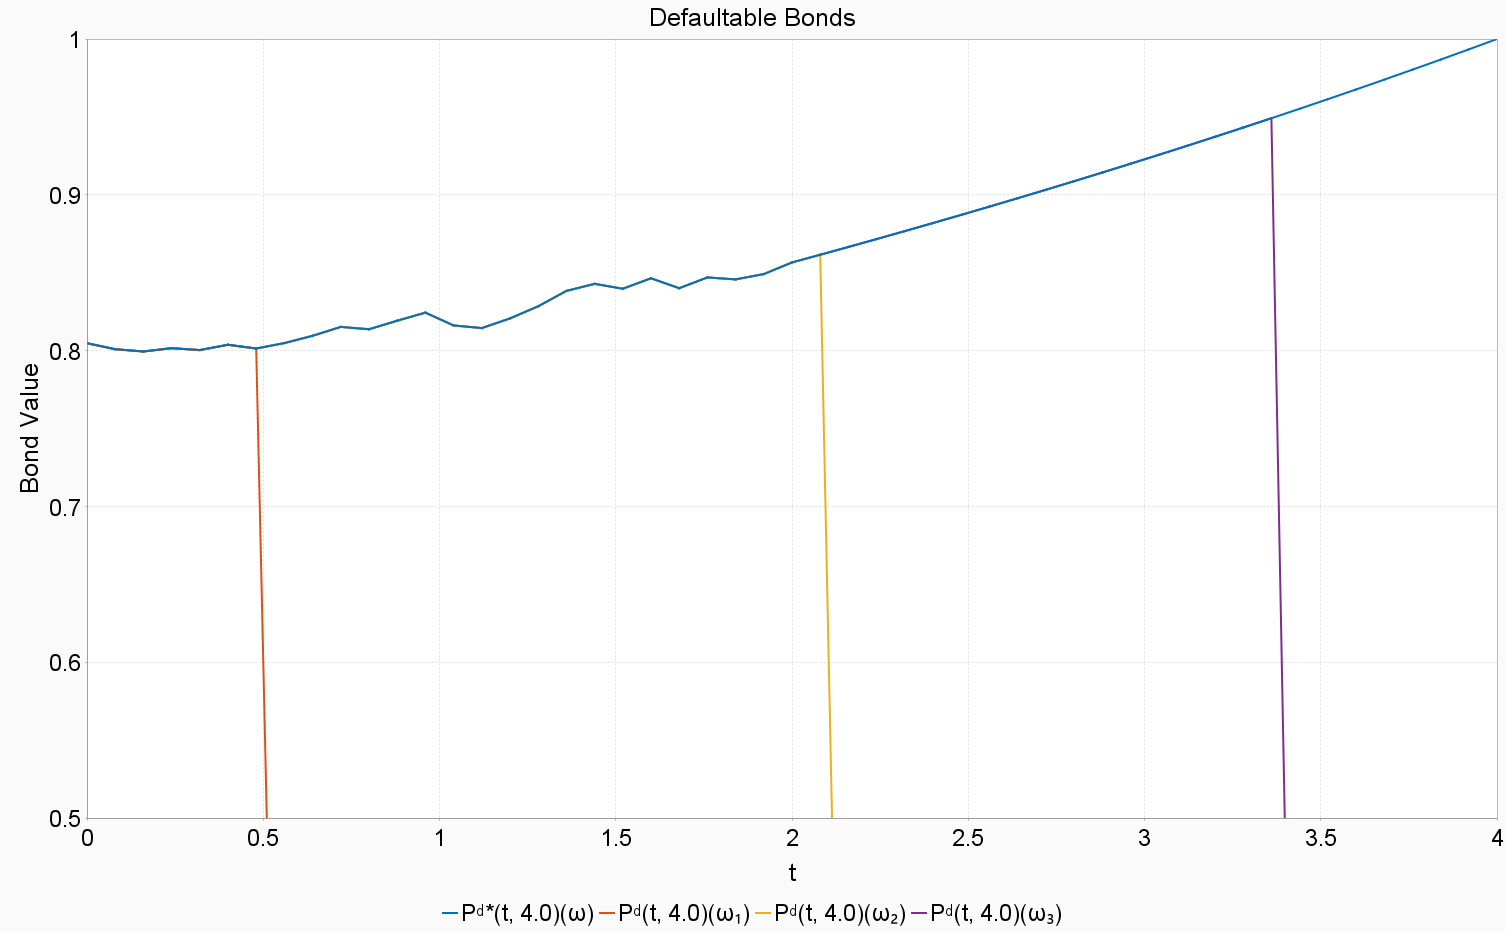
\includegraphics[width=\linewidth]{SurvivalProbability}
		\caption{Paths of $P^d$}
		\label{fig:survivalprobabilityvisualisation}
	\end{figure}
	\\In this example $\mathbb{G}$ captures only the path of $P^{d,*}(t; 4.0)$, which is equal for $\omega = \omega_1, \omega_2$ and $\omega_3$, while $P^d(t; 4.0)(\omega_1) \ne P^d(t; 4.0)(\omega_2) \ne P^d(t; 4.0)(\omega_3)$ for $t = 4.0$.\\
	With this pathwise probability we will now be able to numerically price credits and credit derivatives.
	
	
	
	% -------- Pricing of credits with optionalities
	
	
	\pagebreak
	\section{Loans and Credit Option Pricing}
	In this section we take a look at pricing loans and credit options.
	\subsection{General Loan Pricing}
	Let us first take a look what a loan is in general. "A loan is a sum of money that one or more individuals or companies borrow from banks or other financial institutions [...]. In doing so, the borrower incurs a debt, which he has to pay back with interest and within a given period of time."\cite{corpFinInst}.\\
	In this sense a loan is nothing else than a fixed coupon bond, where the nominal $N$ represents the debt and the coupons $c_i$ represent the interest.
	
	\subsection{Credit Options}
	
	\subsection{Introducing Behavioral Aspects}
	
	
	
	% -------- Implementation of the main model ------------------
	
	
	\pagebreak
	\section{Implementation Details}
	The implementation of the described concepts are a crucial part of this thesis.\\
	We use Java, which is a purely object oriented programming language, for having a good  code readability while still performing very well. We assume a basic knowledge in Java.
	As build system we use Maven.\\
	Before we can jump into any code, though, we need to describe ways to discretize a stochastic process.
	
	\subsection{Numerical Schemes for Stochastic Processes}
	In this chapter we introduce three ways to approach the simulation of stochastic processes described by SDEs. All of these numerical schemes can also be found in \cite{kloedenSchemes}, which is also the main source of this section.\\
	Let us start with the well-known Euler Scheme:
	\begin{definition}
		Let $X=(X_t)_{t\in [0;\tilde{T}]}$ be a $n$-dimensional stochastic process which satisfies:
		\begin{align*}
			dX_t &= \mu(t, X_t)dt + \sigma(t, X_t) \cdot dU_t,\\
			X_0 &= x,
		\end{align*}
		where $U$ is a $d$-dimensional standard Brownian Motion, $\mu: [0;\tilde{T}] \times \mathbb{R}^n \rightarrow \mathbb{R}^n$ and $\sigma: [0;\tilde{T}] \times \mathbb{R}^n \rightarrow \mathbb{R}^{n \times d}$ are functions and $x \in \mathbb{R}^n$.\\
		Furthermore let $m \in \mathbb{N}$, $(t_i)_{i\in \{0, ..., m\}}$, where $0=t_0 < t_1 < ... < t_m=\tilde{T}$.\\
		Then we call the discrete process $\hat{X} = (\hat{X}_{t_i})_{i \in \{0, ..., m\}}$
		\begin{align*}
			\hat{X}_{t_0} &= x,\\
			\hat{X}_{t_{i+1}} &= \hat{X}_{t_{i}} + \mu(t_i, \hat{X}_{t_{i}})\Delta t_i + \sigma(t_i, \hat{X}_{t_{i}}) \cdot \Delta U_{t_i} \quad i \in \{0, ..., m-1\}
		\end{align*}
		the \emph{Euler scheme} of $X$.
	\end{definition}	
	
	
	\subsection{The finMath Library}
	To not start from null, we use the finMath Library of Prof. Christian Fries as starting point for our code basis.\\
	The finMath library is written in Java and provides interfaces and classes for the use in stochastics and financial mathematics.
	\subsubsection{The RandomVariable interface}
	
	\subsection{Implementation of the Defaultable LIBOR Model}
	
	\subsection{Valuation of Financial Products}
	
	
	
	
	
	
	% ------------ Symbol Reference ----------------
	\pagebreak
	\section{List of Symbols}
	\begin{tabular}{cl}
		
		Annotation & Meaning \\
		\hline
		SDE & stochastic differential equation \\
		w.r.t. & with respect to \\
		$\mathbb{Q}^B$ & martingale measure w.r.t. the numeraire $B(t)$\\
		$m(t)$ & For a tenor $T_0 < ... < T_N$, $m(t):= \max\{i \in \{0, ..., N-1\} \; | \; T_i \le t \}$\\
		
	\end{tabular}
	\pagebreak
%	\begin{thebibliography}{}
		
		\bibliographystyle{acm}
		\bibliography{Bibliographie}
		
%		\bibitem{FriesDLMM}
%		Fries, Christian P..
%		2022. 
%		\textit{Defaultable Discrete Forward Rate Model with Covariance Structure guaranteeing Positive Credit Spreads}.
%		Available at SSRN: \texttt{<https://ssrn.com/abstract=3667878>} or \texttt{<http://dx.doi.org/10.2139/ssrn.3667878>}.
%		Last accessed \today.
		
		
%	\end{thebibliography}
	\newpage
	\thispagestyle{empty}
	\clearpage
	
	\section*{Ehrenwörtliche Erklärung}
	
	Ich erkläre hiermit ehrenwörtlich, dass ich die vorliegende Arbeit selbständig angefertigt habe; die aus fremden Quellen direkt oder indirekt übernommenen Gedanken sind als solche kenntlich gemacht.
	\par \bigskip
	\noindent Die Arbeit wurde bisher keiner anderen Prüfungsbehörde vorgelegt und auch noch nicht veröffentlicht.
	
	\vspace{4cm}
	
	\hspace{2cm} Ort, Datum \hfill Unterschrift \hspace{2cm}
	\pagebreak
\end{document}